%%%%%%%%%%%%%%%%%%%%%%%% Chapter 3: Background %%%%%%%%%%%%%%%%%%%%
% Equation (1): Initial Embeddings
% - z_0: The initial sequence of embeddings that will be inputted into the Transformer encoder.
% - x_class: A learnable embedding that represents the classification token, similar to BERT's [class] token.
% - x_p^i: The flattened vector of the i-th image patch.
% - E: The trainable linear projection matrix that maps the flattened image patches into D dimensions.
% - N: The total number of patches into which the image is divided.
% - E_pos: The position embeddings added to the patch embeddings to give the model information about the order of the patches.
% - +: Denotes concatenation of the classification embedding and the patch embeddings, followed by element-wise addition of position embeddings.

% Equation (2): Multiheaded Self-Attention (MSA) and Residual Connection
% - z'_l: The output of the multiheaded self-attention (MSA) block for layer l after adding the residual connection.
% - MSA: Multiheaded self-attention function that allows the model to focus on different parts of the sequence.
% - LN: Layernorm function that normalizes the input across features.
% - z_{l-1}: The output of the previous layer or the initial embeddings for l = 1.

% Equation (3): MLP Block and Residual Connection
% - z_l: The output of the MLP block for layer l after adding the residual connection.
% - MLP: Multilayer perceptron function, which is a feedforward neural network that can model complex functions.
% - LN: Layernorm function applied again to normalize the inputs for the MLP block.
% - z'_l: The output from the self-attention block which serves as an input to the MLP block.

% Equation (4): Final Output Representation
% - y: The final image representation used for classification.
% - LN: The layernorm function applied to the output of the last layer.
% - z_L^0: The output of the Transformer encoder corresponding to the classification token.
% - L: The total number of layers in the Transformer encoder
%%%%%%%%%%%%%%%%%%%%%%%%%%%%%%%%%%%%%%%%%%%%%%%%%%%%%%%%%%%%%%%%%%%
\chapter{Background}
\label{chapter:background}
We looked at the study on driver distraction detection and dataset imbalance in the last chapter. Following the research gaps identified in the previous section and the recommended research alternatives, this chapter will look at the background knowledge and working principles of the algorithms and models employed in this thesis to address the research problems. It covers the working principle of the HDBSCAN clustering algorithm~\citep{HDBSCAN_algo_campello2013density} and vision transformer~\cite{Vit_Paper_Dosovitskiy2020AnII}. Also discussed are the \gls{din}~\citep{dino_caron2021emerging} framework and it's improved version \gls{dino}~\citep{dinov2_oquab2023dinov2} for training vision transformer models.

\section{HDBSCAN Clustering Algorithm}
Clusters can be represented as dense regions in the data space, divided by sparse areas. Density-based clustering algorithms use this strategy to identify non-spherical groupings~\citep{density_based_clustering_book_han2011data}. Density-based clustering detects clusters in data by separating regions of high and low point density ~\citep{density_based_clustering_book_han2011data}. DBSCAN~\citep{DBSCAN_algo_ester1996density} is a type of density based clustering algorithm which groups points that are closely packed together, marking points that are in low-density regions as noise. This method is particularly effective for discovering clusters of arbitrary shapes and sizes in datasets with noise~\citep{hdbscanComparingPython}. While DBSCAN~\citep{DBSCAN_algo_ester1996density} is powerful, it has limitations. It requires two parameters: \textit{eps} (maximum distance between neighbors) and \textit{min\_samples} (minimum number of points to form a dense region)~\citep{DBSCAN_algo_ester1996density, hdbscanComparingPython}. Selecting suitable values for these variables might prove problematic, especially for datasets with varying density~\citep{hdbscanComparingPython}. Moreover, DBSCAN~\citep{DBSCAN_algo_ester1996density} does not inherently provide a way to explore the hierarchical structure of clusters~\citep{hdbscanComparingPython}.

HDBSCAN (Hierarchical Density-Based Spatial Clustering of Applications with Noise)~\citep{HDBSCAN_algo_campello2013density} extends DBSCAN~\citep{DBSCAN_algo_ester1996density} by addressing these limitations. It combines density-based clustering with hierarchical clustering, allowing it to handle data with varying density more effectively and revealing a hierarchy of clusters~\citep{hdbscanComparingPython}.

\newpage

\paragraph{Working of HDBSCAN algorithm:} Based on the~\citep{HDBSCAN_algo_campello2013density, HDBSCAN_2015_campello2015hierarchical} papers, the working of HDBSCAN algorithm can be divided into following steps:

\begin{enumerate}
    \item \textbf{Transforming the Space}:
    \begin{itemize}
        \item HDBSCAN begins by computing the core distance for each point, which represents the distance to its $k$-th nearest neighbor (where $k$ is defined by the \textit{min\_samples} parameter).
        \item It then calculates the mutual reachability distance between pairs of points. This distance accounts for the core distance of the points, ensuring clusters can be identified in regions with varying density.
    \end{itemize}
    
    \item \textbf{Building the Minimum Spanning Tree (MST)}:
    \begin{itemize}
        \item Using the mutual reachability distances, HDBSCAN constructs a minimum spanning tree (MST). This tree connects all points in the dataset with the shortest possible total distance, ensuring every point is reachable from any other point~\citep{hdbscanComparingPython}.
    \end{itemize}
    
    \item \textbf{Condensing the Tree}:
    \begin{itemize}
        \item The MST is condensed into a hierarchy of connected components by progressively removing the edges with the longest mutual reachability distances. This process reveals a tree structure, or dendrogram, that represents clusters at different density levels~\citep{hdbscanComparingPython}.
    \end{itemize}
    
    \item \textbf{Extracting Stable Clusters}:
    \begin{itemize}
        \item From the dendrogram, HDBSCAN uses the Excess of Mass (EOM) method to extract clusters. EOM identifies the most stable clusters by measuring their persistence across different density levels. Stable clusters are those that remain consistent over a range of scales, indicating they are meaningful groupings of data points~\citep{hdbscanComparingPython}.
    \end{itemize}
    
    \item \textbf{Outlier Detection}:
    \begin{itemize}
        \item Points that do not belong to any stable cluster are labeled as noise. These points are in low-density regions and do not fulfill the requirements to be considered as part of a cluster~\citep{HDBSCAN_algo_campello2013density, HDBSCAN_2015_campello2015hierarchical}.
    \end{itemize}
\end{enumerate}

\paragraph{Key Parameters of HDBSCAN:}

\begin{itemize}
    \item \textbf{Minimum Cluster Size (e.g., 25)}: Sets the smallest allowable size for a cluster. Clusters smaller than this are considered noise.
    \item \textbf{min\_samples (e.g., 1)}: Specifies the minimum number of points required within a neighborhood for a point to be classified as a core point, hence affecting the computations of local density~\citep{HDBSCAN_algo_campello2013density, HDBSCAN_2015_campello2015hierarchical, hdbscanComparingPython}.
    \item \textbf{cluster\_selection\_epsilon (0.0)}: Controls the sensitivity for cluster formation. A value of 0.0 applies the strictest criteria.
    \item \textbf{metric (`euclidean')}: Specifies the distance metric, with `euclidean' being the default for calculating distances between points~\citep{hdbscanComparingPython}.
    \item \textbf{cluster\_selection\_method (`eom')}: Determines how clusters are selected from the hierarchical tree, with `eom' favoring stable, persistent clusters.
\end{itemize}

HDBSCAN~\citep{HDBSCAN_algo_campello2013density} improves upon traditional density-based clustering by combining it with hierarchical clustering techniques. It enables the HDBSCAN algorithm to efficiently process datasets with different levels of density, detect clusters of any shape, and identify significant clusters more reliably than techniques such as DBSCAN~\citep{DBSCAN_algo_ester1996density}. Through its use of core distances, mutual reachability distances, and hierarchical extraction methods, HDBSCAN~\citep{HDBSCAN_algo_campello2013density} provides a powerful tool for clustering complex data. While HDBSCAN is relatively less affected by parameter settings compared to other clustering algorithms, it still necessitates the configuration of parameters such as `min\_cluster\_size' and `min\_samples', which can impact the clustering results and is a limitation of this algorithm~\citep{hdbscanComparingPython, HDBSCAN_2015_campello2015hierarchical}.

\section{Vision Transformer}
The \gls{vit}~\citep{Vit_Paper_Dosovitskiy2020AnII}~ has transformed the computer vision domain by demonstrating that \gls{cnn}s~\citep{CNN_o2015introduction} are not necessary for achieving high performance in image classification tasks. ViT applies the Transformer architecture~\citep{Vaswani2017AttentionIA}, originally intended for sequential data in Natural Language Processing (NLP)~\citep{NLP_Book_eisenstein2019introduction}, to process images by considering them as sequences of patches, akin to tokens in text. 

\begin{figure}[h]
\begin{center}
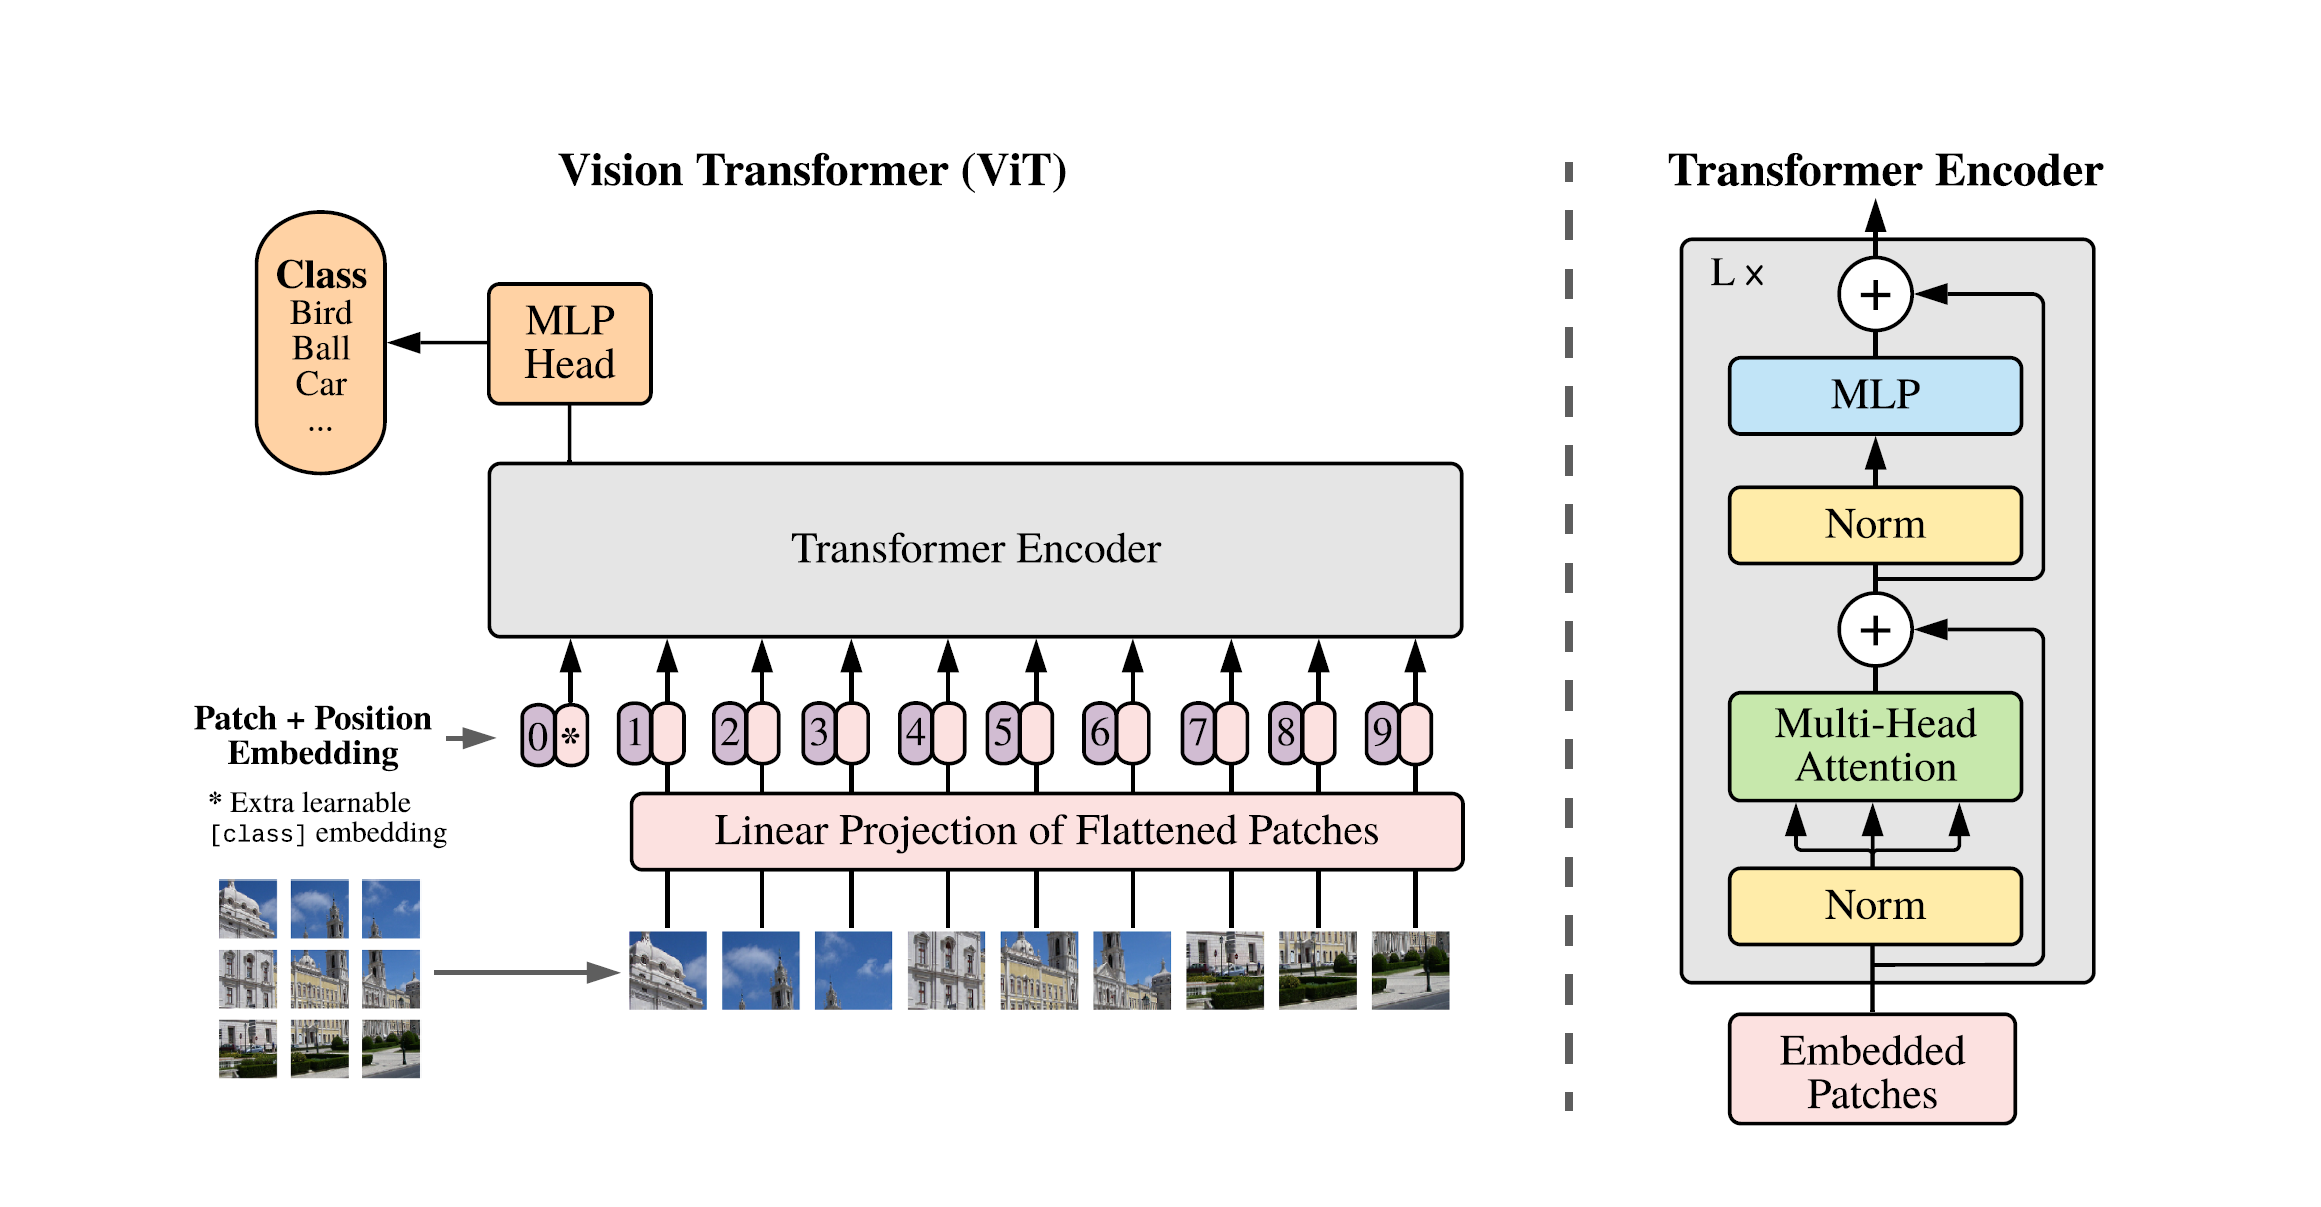
\includegraphics[width=\textwidth]{Vit_arch.png}
\end{center}
\caption[Vision Transformer Architecture]{Vision Transformer Architecture from~\citep{Vit_Paper_Dosovitskiy2020AnII}.}
\label{fig:vit_arch}
\end{figure}

\paragraph{Vision Transformer Architecture:}
The Vision transformer architecture consists of key elements including image patches, patch and positional embedding, learnable class embedding, Transformer Encoder, and MLP Head as shown in figure~\ref{fig:vit_arch}. Image patches are embedded linearly, with position embeddings for spatial information preservation. The transformer encoder is composed of layers that alternate between multi-headed self-attention and MLP blocks. LayerNorm (LN) is applied before each block and residual connections are applied after each block. The MLP blocks have two layers with a GELU non-linearity to maintain local and translational equivariance. The multi-headed self-attention layers record global dependencies across the image~\citep{Vit_Paper_Dosovitskiy2020AnII}.~The MLP Head converts learned features into class output, sometimes it is also referred as the classifier head in classification tasks.

\paragraph{Mathematical Functions and Terminology:}
This paragraph adheres to the notations and conventions established in the Vision Transformer (ViT) paper by~\citet{Vit_Paper_Dosovitskiy2020AnII}. All descriptions and mathematical formulations presented herein are based on those detailed in the original paper.

The process includes transforming image patches into embeddings, adding positional embeddings and a class token, and then passing them through the Transformer encoder, which entails a sequence of essential mathematical operations necessary for understanding the functionality of ViT. The components include linear transformations for patch embedding, softmax normalization in the self-attention mechanism, and the GELU~\citep{GELU_act_fxn_hendrycks2016gaussian} non-linearity in \gls{mlp} blocks.

\citet{Vit_Paper_Dosovitskiy2020AnII} considered an RGB image $\mathbf{x}$ with dimensions $H \times W \times C$, where H represents Height, W represents Width, and C represents the color channel of the image. The image has a resolution of $H \times W$. \citet{Vit_Paper_Dosovitskiy2020AnII} converted this image into a series of 2D image patches by dividing it into $N$ patches with a resolution of $P^2$. 

\citet{Vit_Paper_Dosovitskiy2020AnII} mathematically transformed an image $\mathbf{x}$ into a 2D sequence of image patches $\mathbf{x}_p$, as shown in equation~\ref{equation:3.1}. 

% Centered with equation number
\begin{equation}
\label{equation:3.1}
\mathbf{x} \in \mathbb{R}^{H \times W \times C} \rightarrow \mathbf{x}_p \in \mathbb{R}^{N \times (P^2 \times C)}
\end{equation}
The lowercase letter ``p" represents the patch. The number of patches, N, obtained from this transformation is determined by dividing the resolution of the original image by the resolution of each patch. \citet{Vit_Paper_Dosovitskiy2020AnII} expressed N as the product of H and W divided by P squared as given in equation~\ref{equation:3.2}. 
\begin{equation}
\label{equation:3.2}
N = \frac{H \times W}{P^{2}}
\end{equation}
Afterwards, \citet{Vit_Paper_Dosovitskiy2020AnII} turned the two-dimensional patch sequence into a one-dimensional sequence using linear projections to align with the input requirements of the conventional Transformer encoder~\citep{Vaswani2017AttentionIA}, which only accepts one-dimensional token embeddings. The linearly projected embedding is referred to as Patch embedding and is trainable. 

According to ~\citet{Vit_Paper_Dosovitskiy2020AnII}, the initial patch embeddings and positional encoding of an input image in the Vision Transformer architecture can be defined as:

% \\ for new line and & for concatinationg, \quad for spacing
\begin{equation}
\begin{aligned}
\mathbf{z}_0 & =\left[\mathbf{x}_{\text {class}} ; \mathbf{x}_p^1 \mathbf{E} ; \mathbf{x}_p^2 \mathbf{E} ; \cdots ; \mathbf{x}_p^N \mathbf{E}\right] \\
& \quad +\mathbf{E}_{\text {pos}}, \quad \mathbf{E} \in \mathbb{R}^{\left(P^2 \cdot C\right) \times D}, \quad
\mathbf{E}_{\text {pos}} \in \mathbb{R}^{(N+1) \times D}
\end{aligned}
\label{3.3}
\end{equation}


In equation ~\ref{3.3},~$\mathbf{z}_0$ is the initial embedding matrix input into the Transformer encoder. The image is initially divided into N flattened 2D patches, indicated by $x_{p}^{i}$, where i denotes the count of patches from 1 to N. These patches are then linearly projected into a D-dimensional embedding space using a trainable matrix E~\citep{Vit_Paper_Dosovitskiy2020AnII}. The embedding matrix E is shared by all patches, representing the idea that each patch is equivalent to a `word' in NLP tasks. Position embeddings $\mathbf{E}_{\text {pos }}$ are used to maintain positional information, which is crucial given the Transformer's permutation invariance~\citep{Vit_Paper_Dosovitskiy2020AnII}. A specific class embedding $\mathbf{x}_{\text {class }}$ is prepended to the sequence to serve as a proxy for the overall image representation.


Each Transformer encoder layer comprises a self-attention mechanism~\cite{Vaswani2017AttentionIA}, succeeded by a \gls{mlp}. Mathematically, the self-attention mechanism along with residual connection~\citep{residual_connection_he2016deep} for layer $\ell$ is represented as:

\begin{equation}
\begin{aligned}
\mathbf{z}_{\ell}^{\prime} & =\operatorname{MSA}\left(\operatorname{LN}\left(\mathbf{z}_{\ell-1}\right)\right)+\mathbf{z}_{\ell-1}, & & \ell=1 \ldots L \\
\end{aligned}
\label{3.4}
\end{equation}

In the vision transformer architecture, $\ell$ is a number between 1 and $L$, where $L$ is the maximum number of stacked transformer encoders.~The implementation of the multiheaded self-attention (MSA) function on the layer-normalized embeddings from the preceding layer~ $\mathbf{z}_{\ell-1}$, is illustrated in equation~\ref{3.4}. Subsequently, the result of this combined operation, is added in~$\mathbf{z}_{\ell-1}$~as a residual connection~\citep{residual_connection_he2016deep}, thereby enabling gradient flow~\citep{Vit_Paper_Dosovitskiy2020AnII}. The self-attention mechanism's output~$\mathbf{z}_{\ell}^{\prime}$~ is subsequently passed through a \gls{mlp} in the Transformer encoder block as described in equation~\ref{3.5}:
\begin{equation}
\begin{aligned}
\mathbf{z}_{\ell} & =\operatorname{MLP}\left(\operatorname{LN}\left(\mathbf{z}_{\ell}^{\prime}\right)\right)+\mathbf{z}_{\ell}^{\prime}, & & \ell=1 \ldots L \\
\end{aligned}
\label{3.5}
\end{equation}

The output of the Transformer encoder block is the result of combining the output of the \gls{mlp} with the output of residual connection~\citep{Vit_Paper_Dosovitskiy2020AnII}. The \gls{mlp} comprises two dense layers with a GELU~\citep{GELU_act_fxn_hendrycks2016gaussian} activation function.

Ultimately, equation~\ref{3.6} produces the ultimate output representation of the image, which is subsequently employed for classification purposes.

\begin{equation}
\begin{aligned}
\mathbf{y} & =\operatorname{LN}\left(\mathbf{z}_L^0\right) & &
\end{aligned}
\label{3.6}
\end{equation}

The final image representation, denoted as $y$, is derived by applying layer normalization~\citep{Layer_norm_ba2016layer} to the layer that corresponds to the classification token. This representation $y$ contains the aggregated information from all patches and their interactions as distilled through the various Transformer layers. The Vision Transformer's image classification approach replaces traditional convolutional operations with mechanisms that consider image patches as sequences of data points, akin to words in a sentence. This enables the model to learn contextual relationships throughout the image~\citep{Vit_Paper_Dosovitskiy2020AnII}.

% Attention is a measure of a token's relevance to other tokens, including itself. Key, Value, and Query vectors ar learned by a FFNN. Similarity scores computed from Key, Value and Query. Take softmax of these scores to get attention weights.

\paragraph{Multi-headed Self-Attention Mechanism:}
The primary functionality of ViT relies on self-attention, enabling each patch to attend to every other patch in the image. This mechanism allows the model to prioritize the most pertinent regions of the image for the given task. The multi-headed self-attention~\cite{Vaswani2017AttentionIA} (MHSA) improves the model's ability to understand complex spatial structures and connections by recording several visual components at the same time. The detailed process of self-attention mechanism can be found in paper~\cite{Vaswani2017AttentionIA}, while the mathematical explanation of the Multi-headed Self-Attention mechanism is given in Appendix A of the Vision transformer paper~\cite{Vit_Paper_Dosovitskiy2020AnII}.

\section{Evolution of Self-Supervised Learning in Vision Transformers: From DINO to DINOv2}
DINO stands for ``Self-Distillation with NO labels"~\citep{dino_caron2021emerging}. It is an innovative advancement in self-supervised learning for vision transformers. The \gls{din} framework takes a novel approach to self-supervised learning by merging elements of self-training and knowledge distillation, which have previously been employed to increase feature quality by propagating annotations to unlabeled datasets~\citep{dino_caron2021emerging, _35_kn_distill_hinton2015distilling}. Traditionally, knowledge distillation is teaching a smaller, simpler student network to mimic the behavior of a larger, pre-trained teacher network, therefore compressing knowledge into a more efficient model~\citep{_7_modelcompr_buciluǎ2006model, knowdledge_distill_2017_kim2017transferring, dino_caron2021emerging}. \gls{din} framework innovates by converting this method into what is known as ``self-distillation," in which both the student and the teacher are trained concurrently during the learning phase, with no labeled data. In self-supervised vision transformers, label propagation involves both hard and soft assignments~\citep{_41_pseudo_label_semi_sup_lee2013pseudo,_78_plabel_speech_xu2020iterative,_79_billion_scale_yalniz2019billion, _76_seftraining_xie2020self}, with soft assignments~\citep{_76_seftraining_xie2020self} being particularly matched with knowledge distillation concepts~\citep{_7_modelcompr_buciluǎ2006model,_35_kn_distill_hinton2015distilling}. This strategy has usually concentrated on model compression by training smaller networks to mimic the outputs of bigger ones, as proven by~\citet{_76_seftraining_xie2020self}.

DINO applies these notions to a self-supervised situation in which no true labels are available. Unlike prior techniques, which used a pre-trained, fixed teacher~\citep{_13_big_ssl_chen2020big, _25_SEED_fang2021seed,_63_s2_bnn_shen2021s2,_47_boosting_ssl_KT_noroozi2018boosting}, \gls{din} framework dynamically constructs the teacher during training, making knowledge distillation an inherent component of the learning objective rather than a post-processing step~\citep{dino_caron2021emerging}. This approach is similar to codistillation~\citep{_1_codistillation_anil2018large}, in which both the student and teacher networks share the same architecture; however, in \gls{din}, the teacher network is updated using an exponential moving average~\citep{ema_polyak1992acceleration} of the student's parameters rather than mutual distillation as depicted in the figure~\ref{fig:dino_v1_arch}~\citep{dino_caron2021emerging}.

\begin{figure}[h]
\begin{center}
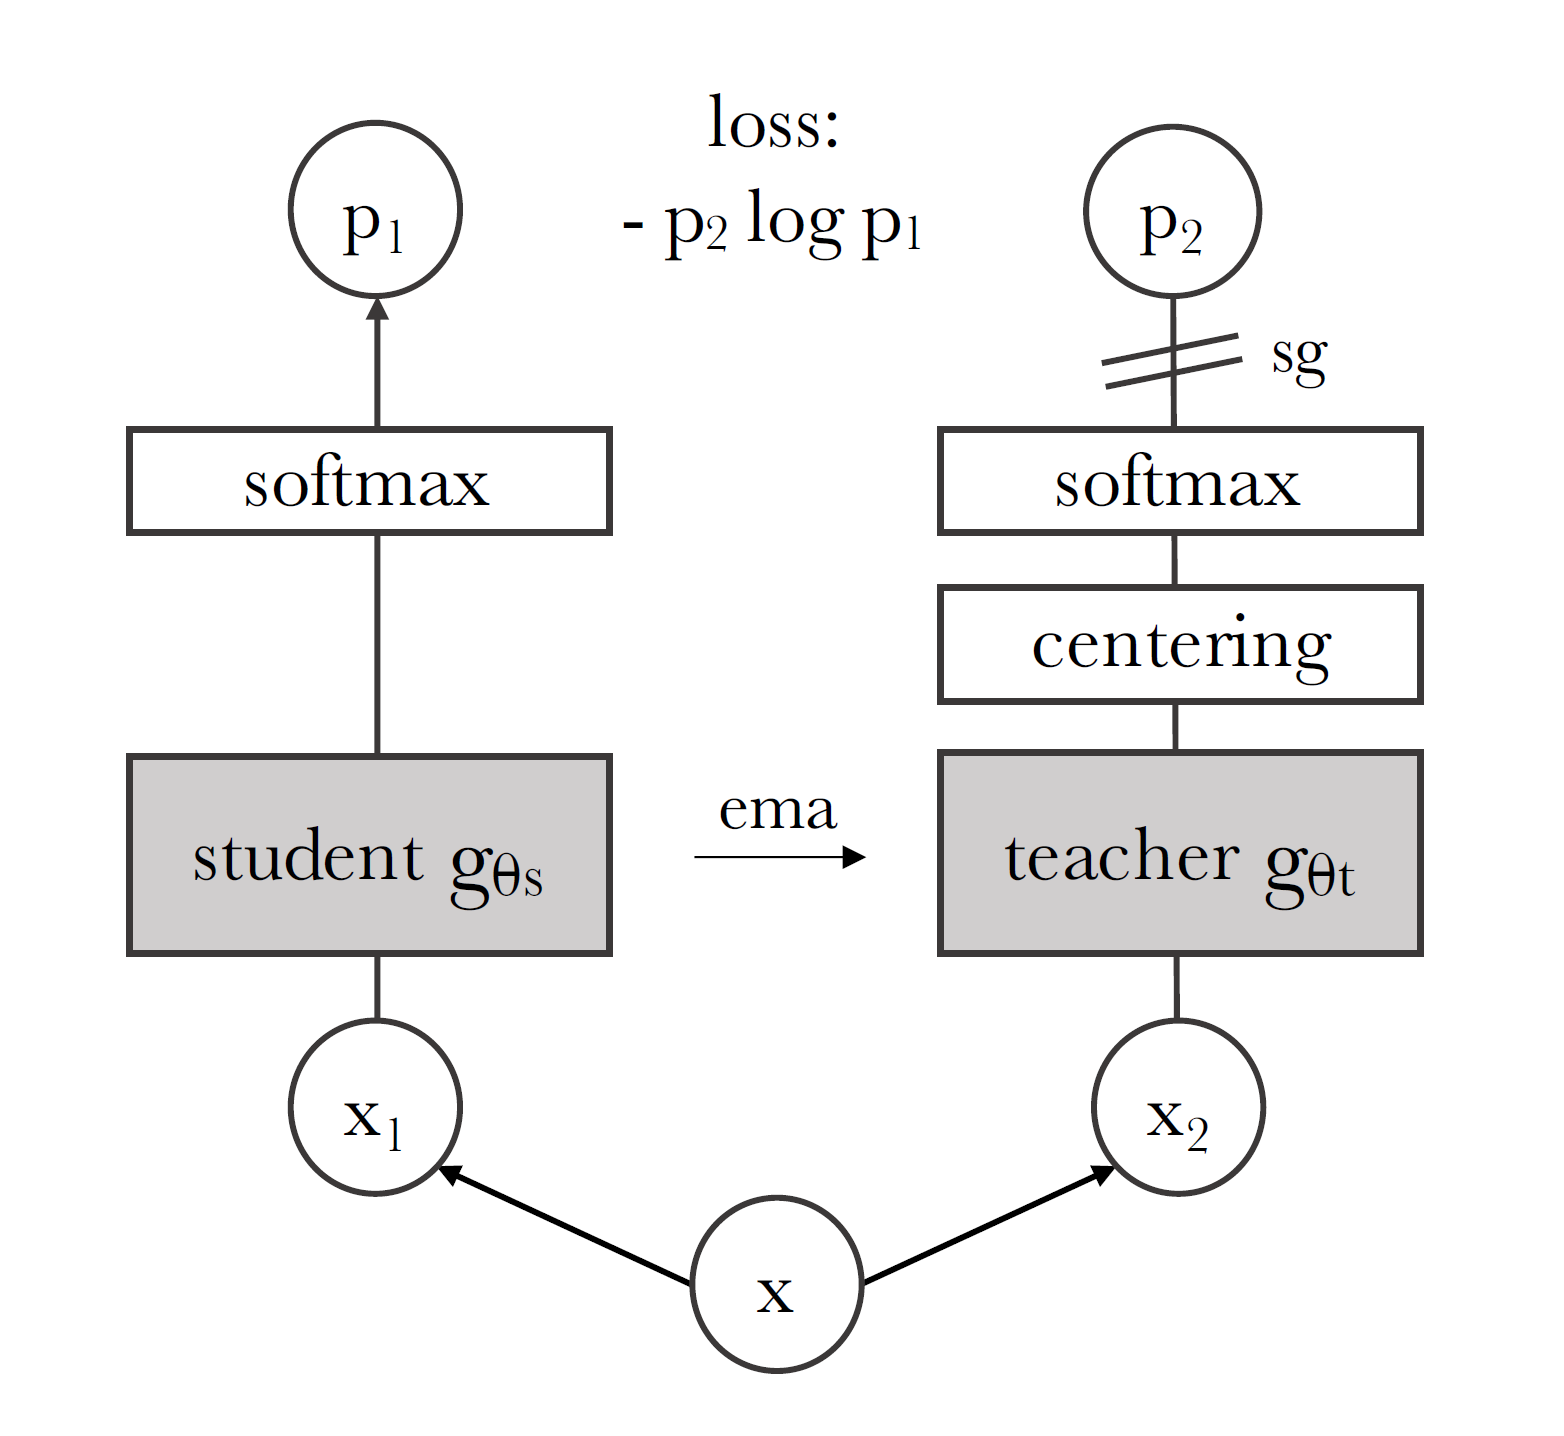
\includegraphics[width=0.5\textwidth]{Images_Thesis/dino_arch_v1.png}
\end{center}
\caption[Self Distillation with no labels]{ A diagram illustrating DINO with one image pair (x1, x2). The image undergoes two random transformations and is passed to both student and teacher networks, which have the same architecture but different parameters. The teacher's output is centered using the batch mean. Both outputs are normalized with temperature softmax and compared using cross-entropy loss. A stop-gradient operator is applied to the teacher, and its parameters are updated using an exponential moving average of the student's parameters~\citep{dino_caron2021emerging}.}
\label{fig:dino_v1_arch}
\end{figure}

The implementation of \gls{din}, as depicted in the figure~\ref{fig:dino_v1_arch}, employs two different random transformations of an input image, extracted from a single input image. These views are then processed by student and teacher networks, which have the same architecture but different parameters. The networks generate K-dimensional features that are normalized using a softmax function controlled by a temperature parameter. The similarity between these features is evaluated using cross-entropy loss. A stop-gradient operation is applied to the teacher to ensure that only the student is directly trained, enhancing the focus on feature generation without direct label dependence. For a comprehensive understanding of the implementation, interested readers can refer to section 3 of the DINO paper~\citep{dino_caron2021emerging}, which provides a complete mathematical foundation and explanation. This thesis focuses specifically on utilizing a pre-trained self-supervised vision transformer encoder to detect driver distraction on the \gls{daa} image dataset. The evaluation procedure used is a linear evaluation protocol.

The DINO architecture has significant implications for Vision Transformers~\citep{Vit_Paper_Dosovitskiy2020AnII} since it has the ability to provide novel qualities to \gls{vit}s, which have primarily been compared to classical \gls{cnn}s. The \gls{din} framework aims to assess the potential benefits of self-supervised \gls{vit}s, including the ability to explicitly describe semantic segmentation and perform successful k-NN classification directly from the features~\cite{dino_caron2021emerging}. In contrast to supervised \gls{vit}s and classical \gls{cnn}s, which do not naturally prioritize certain characteristics, DINO approach stands out and provides remarkable accuracy on ImageNet~\citep{Imagenet1k_ILSVRC15, Imagenet_21K_ridnik2021imagenet} dataset without the need for finetuning~\cite{dino_caron2021emerging}.

\paragraph{Self-Distillation with NO labels Version 2~(DINOv2):}
Building on the fundamental ideas of \gls{din}~\cite{dino_caron2021emerging}, the architecture and training technique are enhanced and refined in various ways in \gls{dino}~\cite{dinov2_oquab2023dinov2}. The architecture of \gls{dino} signifies a significant progression in self-supervised learning in the field of computer vision. It integrates discriminative learning techniques to enhance feature extraction and improve model performance. The \gls{dino} architecture is centered around a dual approach that consists of a student and a teacher network as introduced intially in the \gls{din} paper~\cite{dino_caron2021emerging}. This modified approach utilizes self-distillation techniques to promote strong feature learning without the need for labeled data~\cite{dinov2_oquab2023dinov2}.

The fundamental enhancements in the \gls{dino} architecture consist of:
\begin{itemize}
    \item \textbf{Discriminative Self-supervised Pre-training:}  \gls{dino} utilizes a novel combination of loss functions from \gls{din}~\cite{dino_caron2021emerging} and \gls{ibot}~\citep{_ibot_image_bert_zhou2021ibot}, integrated with the centering mechanism from \gls{swav}~\citep{_SwAV_caron2020unsupervised}. This configuration aids in stabilizing the feature space, preventing the trivial solutions often encountered in self-supervised learning scenarios~\citep{dinov2_oquab2023dinov2}.
    \item \textbf{Dual-Objective Learning:}
        \begin{itemize}
            \item \textbf{Image-level Objective~\cite{dino_caron2021emerging}:} At this level, \gls{dino} framework applies a cross-entropy loss between the outputs of the student and the teacher networks, derived from the class token of a Vision Transformer~\citep{Vit_Paper_Dosovitskiy2020AnII} model. The outputs are obtained from different crops of the same image, encouraging the model to recognize and learn consistent features across varied perspectives and scales~\citep{dino_caron2021emerging, dinov2_oquab2023dinov2}.
            \item \textbf{Patch-level Objective~\citep{_ibot_image_bert_zhou2021ibot}:} This objective introduces variability in the input by masking some patches presented to the student network, but not to the teacher. A cross-entropy loss is then computed between the patch features from both networks. This added complexity ensures the model captures detailed textural and structural information at finer granularities, thus enhancing its overall sensitivity to image content~\citep{dinov2_oquab2023dinov2}. 
        \end{itemize}
    \item \textbf{Adaptive Weight Management:} To optimize learning at different scales, \gls{dino} employs a strategy of untying the head weights for the image-level and patch-level objectives. This approach corrects the tendency of the model to underfit at the patch level or overfit at the image level, thereby balancing the learning focus and improving outcomes at both scales~\citep{dinov2_oquab2023dinov2}. 
    \item \textbf{Sinkhorn-Knopp Centering~\citep{_SwAV_caron2020unsupervised}:} The DINOv2 architecture adopts the Sinkhorn-Knopp (SK) algorithm for batch normalization~\citep{_SwAV_caron2020unsupervised} from \gls{swav} framework, a method initially suggested for the \gls{din} and \gls{ibot} framework by \citet{ruan2022weighted}. This algorithm, recommended for its efficiency in normalizing features, replaces the softmax centering typically used in DINO and iBOT setups~\citep{ruan2022weighted}. The SK centering is applied in three iterative steps, mainly for the teacher network, while the student employs softmax normalization. This element helps in maintaining a uniform distribution of features across batches, crucial for consistent self-supervised learning~\citep{dinov2_oquab2023dinov2}.
    \item \textbf{Regularization and High-Resolution Training Phase:} In addition to these structural components, \gls{dino} incorporates KoLeo regularizer~\citep{_koleo_sablayrolles2018spreading} to ensure a diverse spread of features across the learning process and introduces a short high-resolution training phase. These enhancements allow the model to adapt better to high-resolution tasks, which are particularly relevant in contexts such as detailed image analysis, segmentation, and object detection~\citep{dinov2_oquab2023dinov2}.
\end{itemize}

The primary distinctions between DINO and DINOv2 are outlined below:

\textbf{Loss Function Integration:}
    \begin{itemize}
        \item DINO: Introduced knowledge distillation emphasizing feature invariance across various perspectives of the same image~\citep{dino_caron2021emerging}.
        \item DINOv2: Integrated a combination of \gls{din} and \gls{ibot} loss functions, along with the centering techniques from \gls{swav}, to stabilize the learning process further~\citep{dinov2_oquab2023dinov2}.
    \end{itemize}
\textbf{Objective Functions:}
    \begin{itemize}
        \item DINO: Primarily focused on image-level objectives to encourage feature learning across different augmentations of input data~\citep{dino_caron2021emerging}.
        \item DINOv2: Introduced patch-level objectives alongside image-level objectives, involving masking some image patches for the student but not for the teacher, adding complexity and encouraging more detailed feature learning~\citep{dinov2_oquab2023dinov2}.
    \end{itemize}
\textbf{Weight Management:}
    \begin{itemize}
        \item DINO: Did not explicitly address weight tying between different objectives.
        \item DINOv2: Improved the architecture by untying the weights between image-level and patch-level objectives, enhancing model performance across different scales and preventing overfitting or underfitting~\citep{dinov2_oquab2023dinov2}.
    \end{itemize}


\paragraph{Evaluation Protocols for SSL Models}
The evaluation of self-supervised learning \gls{ssl} models, such as our DINOv2-based ViT encoder~\citep{dinov2_oquab2023dinov2}, deviates substantially from conventional supervised approaches. The methods of evaluation for \gls{ssl} models are essential for determining their effectiveness in downstream tasks like driver distraction detection, as these models are generally evaluated based on their capacity to generate valuable representations without direct supervision. 

\paragraph{Types of SSL Evaluation:}
\begin{enumerate}
    \item \textbf{K-Nearest Neighbors (KNN):}
    In the context of \gls{ssl}, a KNN classifier~\citep{kNN_Mucherino2009} uses $\displaystyle l_2$-normalized features extracted by the model to classify new images based on the closest training examples in feature space. This method is advantageous due to its simplicity, speed, and minimal hyperparameter tuning, making it an ideal quick benchmark for SSL models \citep{dino_caron2021emerging, ssl_codebook_balestriero2023cookbook}.

    \item \textbf{Linear Evaluation:}
    The most popular method for evaluating \gls{ssl} models is the linear evaluation, or linear probing. This method tests the quality of the backbone directly, as the linear classifier has limited capacity to adjust to the data, thereby providing a clear signal of the representational power of the underlying parameters. Typically, this involves appending a linear layer to the frozen backbone and optimizing it for several epochs (usually around 100), which is computationally efficient \citep{ssl_zhang_2016_colorful,ssl_zhang_2017split,ssl_codebook_balestriero2023cookbook,ssl_beit_bert_bao2021beit}.

    \item \textbf{Full Fine-Tuning:}
    This method involves training the entire model (both the pre-trained backbone and the newly added classifier) on a downstream task such as driver distraction detection. It is the most thorough evaluation, allowing the model to fully adapt to the new task. However, it is also the most computationally expensive and may not always correlate with the strength of the initial \gls{ssl} pre-training, especially in scenarios where the downstream task is substantially different from the pre-training setup \citep{masked_ae_he2021masked, ssl_codebook_balestriero2023cookbook}.

    \item \textbf{Multi-Layer Perceptron (MLP) Probing:}
    While less common, MLP probing involves adding a small multi-layer perceptron on top of the frozen features. This can reveal whether the features are non-linearly separable, which may be masked by simpler linear probing. However, this approach is more prone to overfitting and typically requires careful management of model capacity and training duration \citep{ssl_bordes2023towards, ssl_codebook_balestriero2023cookbook}.
\end{enumerate}
